\documentclass[a4paper,9pt]{beamer}
\usetheme{Malmoe}  % Base theme
% Now we try to put MILA's colors
\definecolor{MilaBlue1}{RGB}{78,179,225} % lighter, PMS 306
\definecolor{MilaBlue2}{RGB}{35,154,204} % darker, PMS 639

\setbeamercolor{structure}{fg=MilaBlue2}
\setbeamercolor{title}{fg=MilaBlue1,bg=black}
\setbeamercolor{section in head/foot}{fg=MilaBlue1,bg=black}
\setbeamercolor{subsection in head/foot}{fg=MilaBlue2,bg=white}
\setbeamercolor{frametitle}{fg=white,bg=MilaBlue2}

\setbeamertemplate{footline}[page number]
\usepackage[utf8]{inputenc}
\usepackage{url}
\usepackage{minted}

\usepackage[T1]{fontenc}
\usepackage{inconsolata}

% for copy-pastable ', we need the following
\usepackage{upquote}
\usepackage{textcomp}

%\usepackage{ragged2e}
%\usepackage{multirow}
%\usepackage{fancyvrb}
%\usepackage{color}
\def\imagetop#1{\vtop{\null\hbox{#1}}}

% Standard LaTeX stuff - note the optional abbreviated title being provided

%% ALL that presentation slide are not used! We use a normal frame for that.
\title[Theano]{Theano}
\subtitle{A Fast Python Library for Modelling and Training}
\author[Kaushal Kishore]{%
Kaushal Kishore\\
8th Semester, B. Tech (CSE) \\
Indian Institute of Technology, Palakkad\\
Intern - Digital Horizons}

\date{%
April 28th, 2020, New Delhi%
}

\setbeamertemplate{navigation symbols}{}


\begin{document}

\begin{frame}[plain]
  \titlepage
  
\includegraphics[width=1in]{theano.png}
  \hfill
  
\includegraphics[width=1in]{theano.png}
\end{frame}


\subsection*{Instructions}

\subsection*{Objectives}
\begin{frame}[fragile]{Objectives}
  This tutorial will have 5 parts:
  \begin{itemize}
    \item Introduction to Theano -- Motivation and design
    \item Symbolic Expressions
    \item Fuction compilation
    \item Optimized Execution
    \item Case study -- Logistic Regression
  \end{itemize}

% All the material is online at \url{github.com/mila-udem/summerschool2017}

%   \begin{block}{Hands-on examples}
%   Go to \url{http://mila.umontreal.ca/vmip}
%   \begin{itemize}
%     \item Jupyter notebooks
%     \item Executed on AWS instances with a GPU (K80)
%   \end{itemize}
%   \end{block}
\end{frame}


\section{Motivation and design}
\begin{frame}
  \tableofcontents[currentsection]
\end{frame}

\subsection{Goals}

\begin{frame}{Goals}

  \begin{block}{Expressing models as mathematical expressions}
  \begin{itemize}
    \item Not only a collection of standard layers or modules
    \item Not only regular gradient descent
    \item From an interpreted / scripting language
  \end{itemize}
  \end{block}

  \begin{block}{Automatically deriving gradients}
  \begin{itemize}
    \item Define gradients for basic, elementary operations
    \item Treat those gradients as mathematical expressions as well
    \item Simplify automatically the resulting expression
  \end{itemize}
  \end{block}

  \begin{block}{Training the model efficiently}
  \begin{itemize}
    \item Without having to write C / C++ / CUDA code
    \item Automatic simplification of the graph
    \item Automatic code generation
  \end{itemize}
  \end{block}

\end{frame}

\subsection{Design}

\begin{frame}{Theano: A mathematical symbolic expression compiler}

  \begin{block}{Easy to define expressions}
    \begin{itemize}
      \item Using Python
      \item Expressions mimic NumPy's syntax and semantics
    \end{itemize}
  \end{block}

  \begin{block}{Possible to manipulate those expressions}
    \begin{itemize}
      \item Substitutions
      \item Gradient, R operator
      \item Stability optimizations
    \end{itemize}
  \end{block}

  \begin{block}{Fast to compute values for those expressions}
    \begin{itemize}
      \item Speed optimizations
      \item Use fast back-ends (CUDA, BLAS, custom C code)
      \item Inplace optimizations to reduce memory usage
    \end{itemize}
  \end{block}

  Tools to inspect and check for correctness
\end{frame}

\begin{frame}{Theano}
Theano is a Python library that lets you to define, optimize, and evaluate mathematical expressions, especially ones with multi-dimensional arrays (\texttt{numpy.ndarray}). Using Theano it is possible to attain speeds rivaling hand-crafted C implementations for problems involving large amounts of data. It can also surpass C on a CPU by many orders of magnitude by taking advantage of recent GPUs.
\end{frame}


\subsection{Status}

\begin{frame}[fragile]{Current status}
  \begin{itemize}
    \item Mature: developed and used since January 2008 (12 years old)
    \item Theano 1.0 released in November 2017
    \item Driven > 1000 research papers
    \item Many contributors (332 for version 1.0)
    \item Active mailing list with participants worldwide
    \item Used to teach university classes
    \item Core technology for Silicon Valley start-ups
    \item Used for research at large companies
  \end{itemize}
  Theano: \url{deeplearning.net/software/theano/}

  Deep Learning Tutorials: \url{deeplearning.net/tutorial/}
\end{frame}

\begin{frame}{Related projects}
  Many libraries are built on top of Theano (mostly machine learning)
  \begin{itemize}
    \item Blocks
    \item Keras
    \item Lasagne
    \item rllab
    \item PyMC 3
    \item \ldots
  \end{itemize}
  For parallelism
  \begin{itemize}
    \item Platoon
    \item Theano-MPI
    \item Synkhronos
    \item Elephas (through Keras)
  \end{itemize}
\end{frame}


\section{Symbolic expressions}
\begin{frame}
  \tableofcontents[currentsection]
\end{frame}

\begin{frame}{Overview}
  Theano defines a {\bf language}, a {\bf compiler}, and a {\bf library}.
  \begin{itemize}
    \item Define a symbolic expression
    \item Compile a function that can compute values
    \item Execute that function on numeric values
  \end{itemize}
\end{frame}

\begin{frame}[fragile]{Sneak Peek}

    \begin{minted}[fontfamily=tt]{python}
import theano
from theano import tensor
# declare two symbolic floating-point scalars
a = tensor.dscalar()
b = tensor.dscalar()
# create a simple expression
c = a + b
# convert the expression into a callable object that takes (a,b)
# values as input and computes a value for c
f = theano.function([a,b], c)
# bind 1.5 to 'a', 2.5 to 'b', and evaluate 'c'
assert 4.0 == f(1.5, 2.5)
    \end{minted}
\end{frame}

\begin{frame}[fragile]{Sneak Peek}
Theano is not a programming language in the normal sense because you write a program in Python that builds expressions for Theano. Still it is like a programming language in the sense that you have to
\begin{itemize}
    \item declare variables (a,b) and give their types
    \item build expressions for how to put those variables together
    \item compile expression graphs to functions in order to use them for computation.
\end{itemize}

It is good to think of \texttt{theano.function} as the interface to a compiler which builds a callable object from a purely symbolic graph. One of Theano’s most important features is that \texttt{theano.function} can optimize a graph and even compile some or all of it into native machine instructions.
    
\end{frame}

\subsection{Declaring inputs}
\begin{frame}[fragile]{Symbolic inputs}
  Symbolic, strongly-typed inputs
  \begin{minted}[fontfamily=tt]{python}
import theano
from theano import tensor as T
x = T.vector('x')
y = T.vector('y')
  \end{minted}

  \begin{itemize}
    \item All Theano variables have a type
    \item For instance \verb|ivector|, \verb|fmatrix|, \verb|dtensor4|
    \item ndim, dtype, broadcastable pattern, device are part of the type
    \item shape and memory layout (strides) are {\bf not}
  \end{itemize}
\end{frame}


\begin{frame}[fragile]{Shared variables}
  \begin{minted}[fontfamily=tt]{python}
import numpy as np
np.random.seed(42)
W_val = np.random.randn(4, 3)
b_val = np.ones(3)

W = theano.shared(W_val)
b = theano.shared(b_val)
W.name = 'W'
b.name = 'b'
  \end{minted}
  \begin{itemize}
    \item Symbolic variables, with a \textbf{value} associated to them
    \item The value is \textbf{persistent} across function calls
    \item The value is \textbf{shared} among all functions
    \item The value can be \textbf{updated}
  \end{itemize}
\end{frame}

\subsection{Defining expressions}
\begin{frame}[fragile]{Build an expression}
  NumPy-like syntax
  \begin{minted}{python}
dot = T.dot(x, W)
out = T.nnet.sigmoid(dot + b)

C = ((out - y) ** 2).sum()
C.name = 'C'
  \end{minted}

  \begin{itemize}
    \item This creates new \emph{variables}
    \item Outputs of mathematical operations
    \item Graph structure connecting them
  \end{itemize}
\end{frame}

\begin{frame}{\texttt{pydotprint(out, compact=False)}}
    \center
    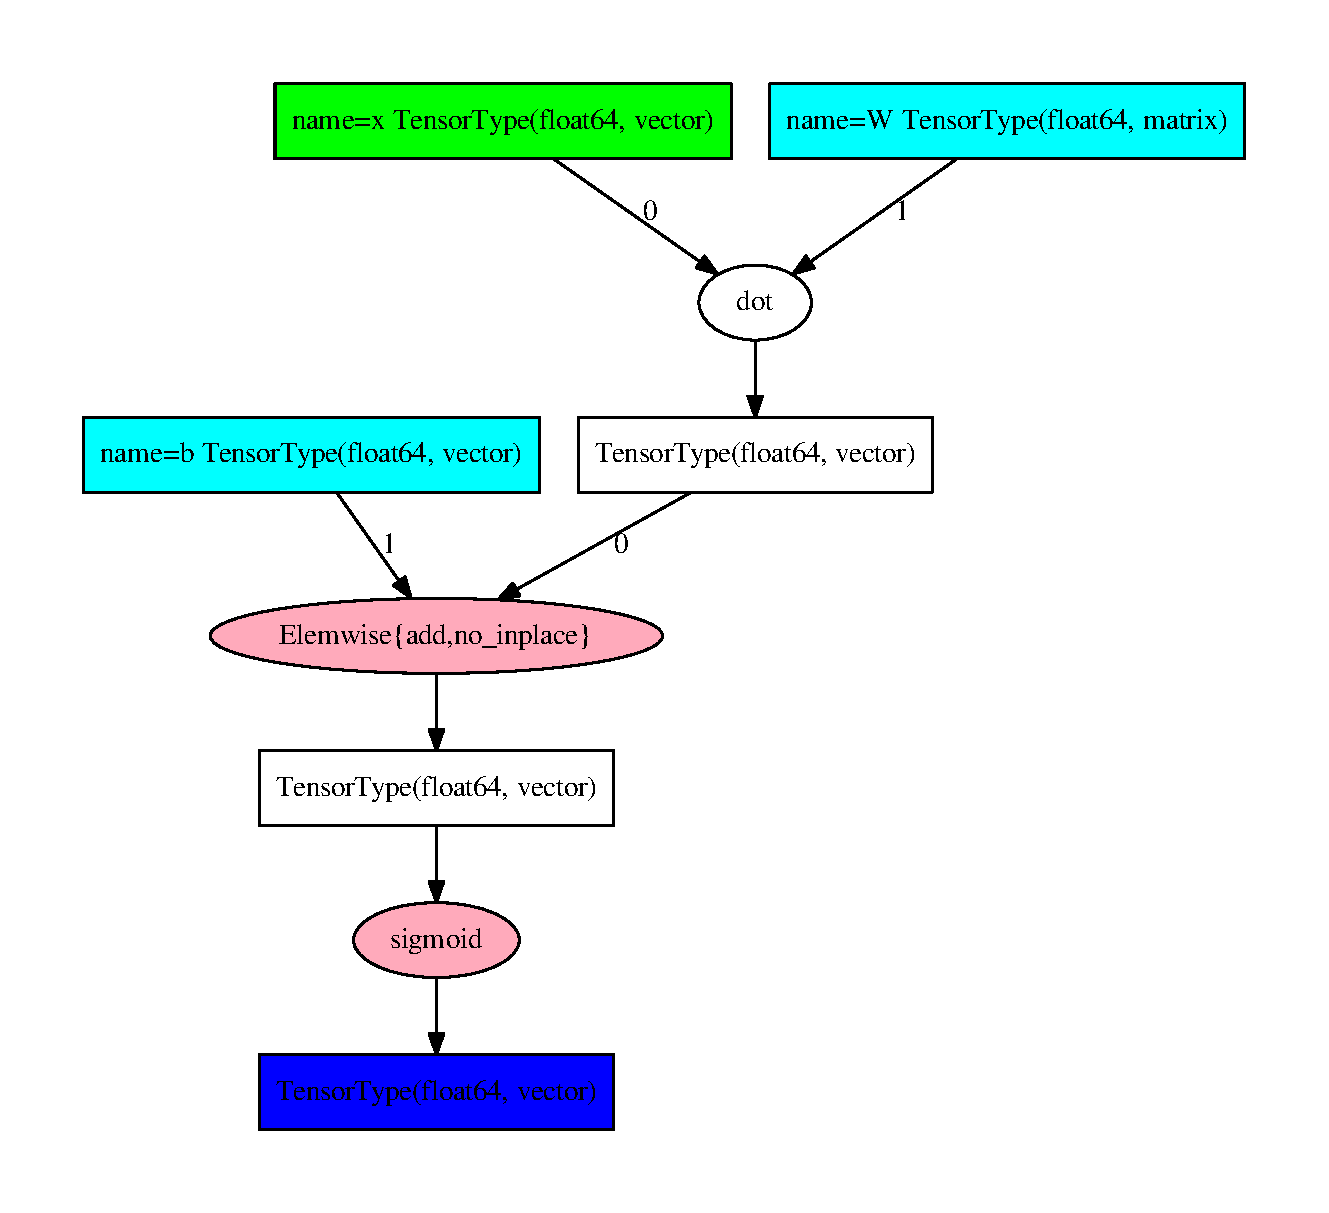
\includegraphics[height=0.9\textheight]{pydotprint_out_long.pdf}
\end{frame}

\begin{frame}{\texttt{pydotprint(out)}}
    \center
    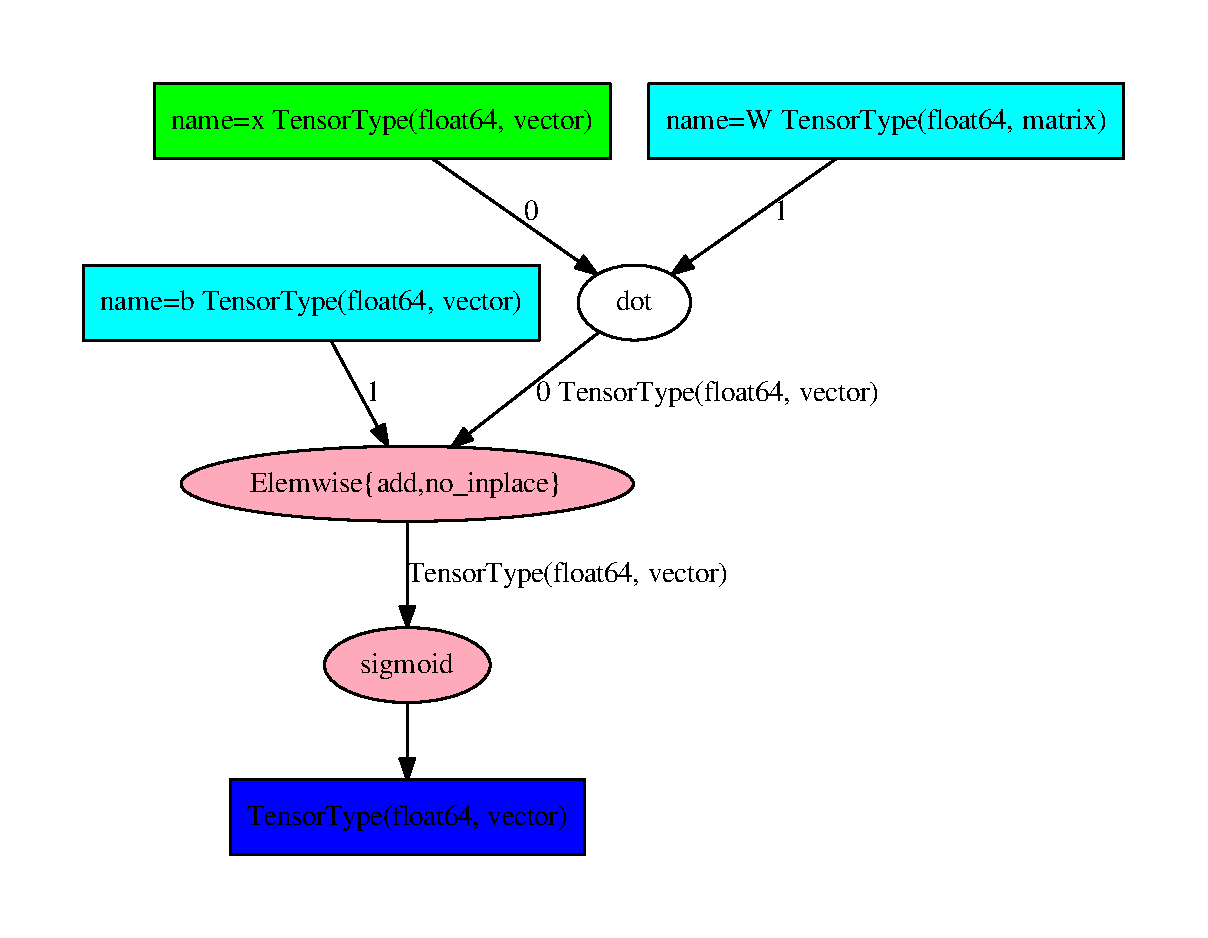
\includegraphics[height=0.9\textheight]{pydotprint_out.pdf}
\end{frame}

\subsection{Deriving gradients}
\begin{frame}{The back-propagation algorithm}
  Application of the chain-rule for functions from ${\mathbb R}^N$ to ${\mathbb R}$.
  \begin{itemize}
    \item $C: {\mathbb R}^N \rightarrow {\mathbb R}$
    \item $f: {\mathbb R}^M \rightarrow {\mathbb R}$
    \item $g: {\mathbb R}^N \rightarrow {\mathbb R}^M$
    \item $C(x) = f(g(x))$
    \item $\left.\frac{\partial C}{\partial x}\right|_x =
              \left.\frac{\partial f}{\partial g}\right|_{g(x)}
              \cdot \left.\frac{\partial g}{\partial x}\right|_x$
  \end{itemize}
%   The whole $M \times N$ Jacobian matrix $\left.\frac{\partial g}{\partial x}\right|_x$
%   is not needed.

%   We only need $\nabla g_x: {\mathbb R}^M \rightarrow {\mathbb R}^N, v \mapsto v \cdot \left.\frac{\partial g}{\partial x}\right|_x$

%   This is implemented for (almost) each mathematical operation in Theano.
\end{frame}

\begin{frame}[fragile]{Using \texttt{theano.grad}}
\verb|theano.grad| traverses the graph, applying the chain rule.
  \begin{minted}{python}
dC_dW = theano.grad(C, W)
dC_db = theano.grad(C, b)
# or dC_dW, dC_db = theano.grad(C, [W, b])
  \end{minted}
  \begin{itemize}
    \item \verb|dC_dW| and \verb|dC_db| are symbolic expressions, like \verb|out| and \verb|C|
    \item There are no numerical values at this point
    \item They are part of the same computation graph
    \item They can also be used to build new expressions
  \end{itemize}
  \begin{minted}{python}
upd_W = W - 0.1 * dC_dW
upd_b = b - 0.1 * dC_db
  \end{minted}
\end{frame}

\begin{frame}{\texttt{pydotprint([dC\_dW, dC\_db])}}
    \center
    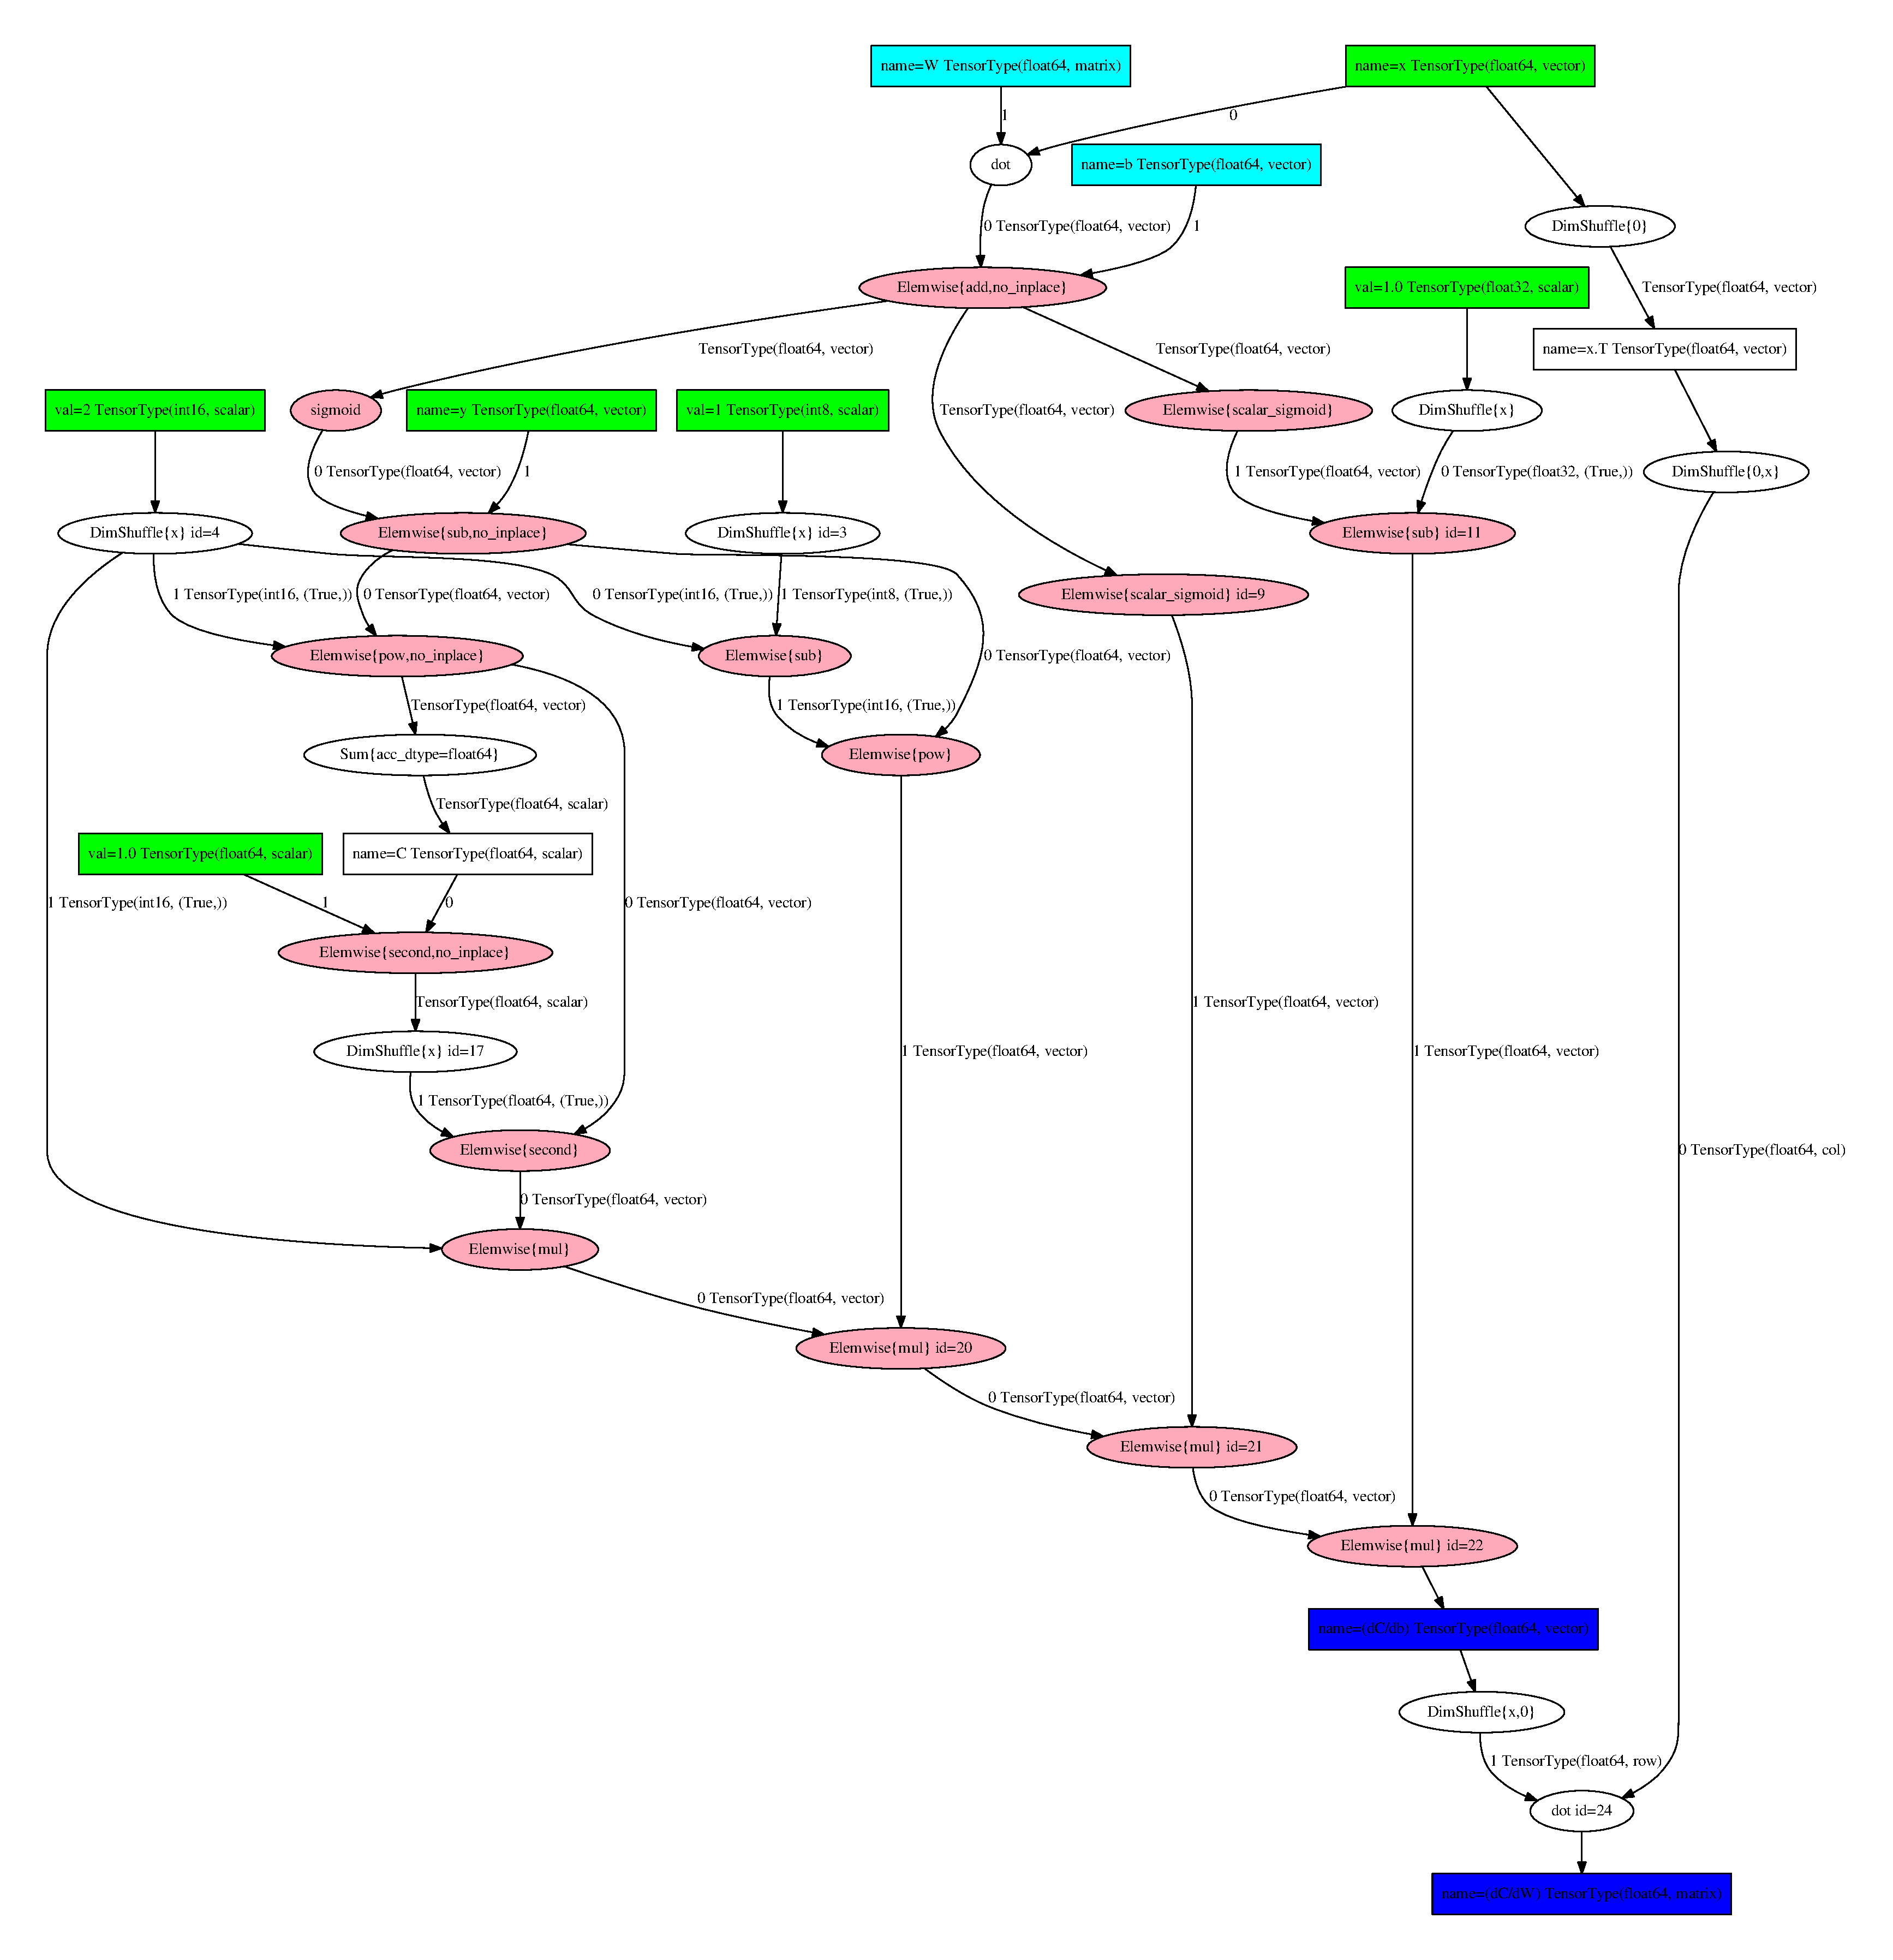
\includegraphics[height=0.9\textheight]{pydotprint_grad.pdf}
\end{frame}

\begin{frame}{\texttt{pydotprint([upd\_W, upd\_b])}}
    \center
    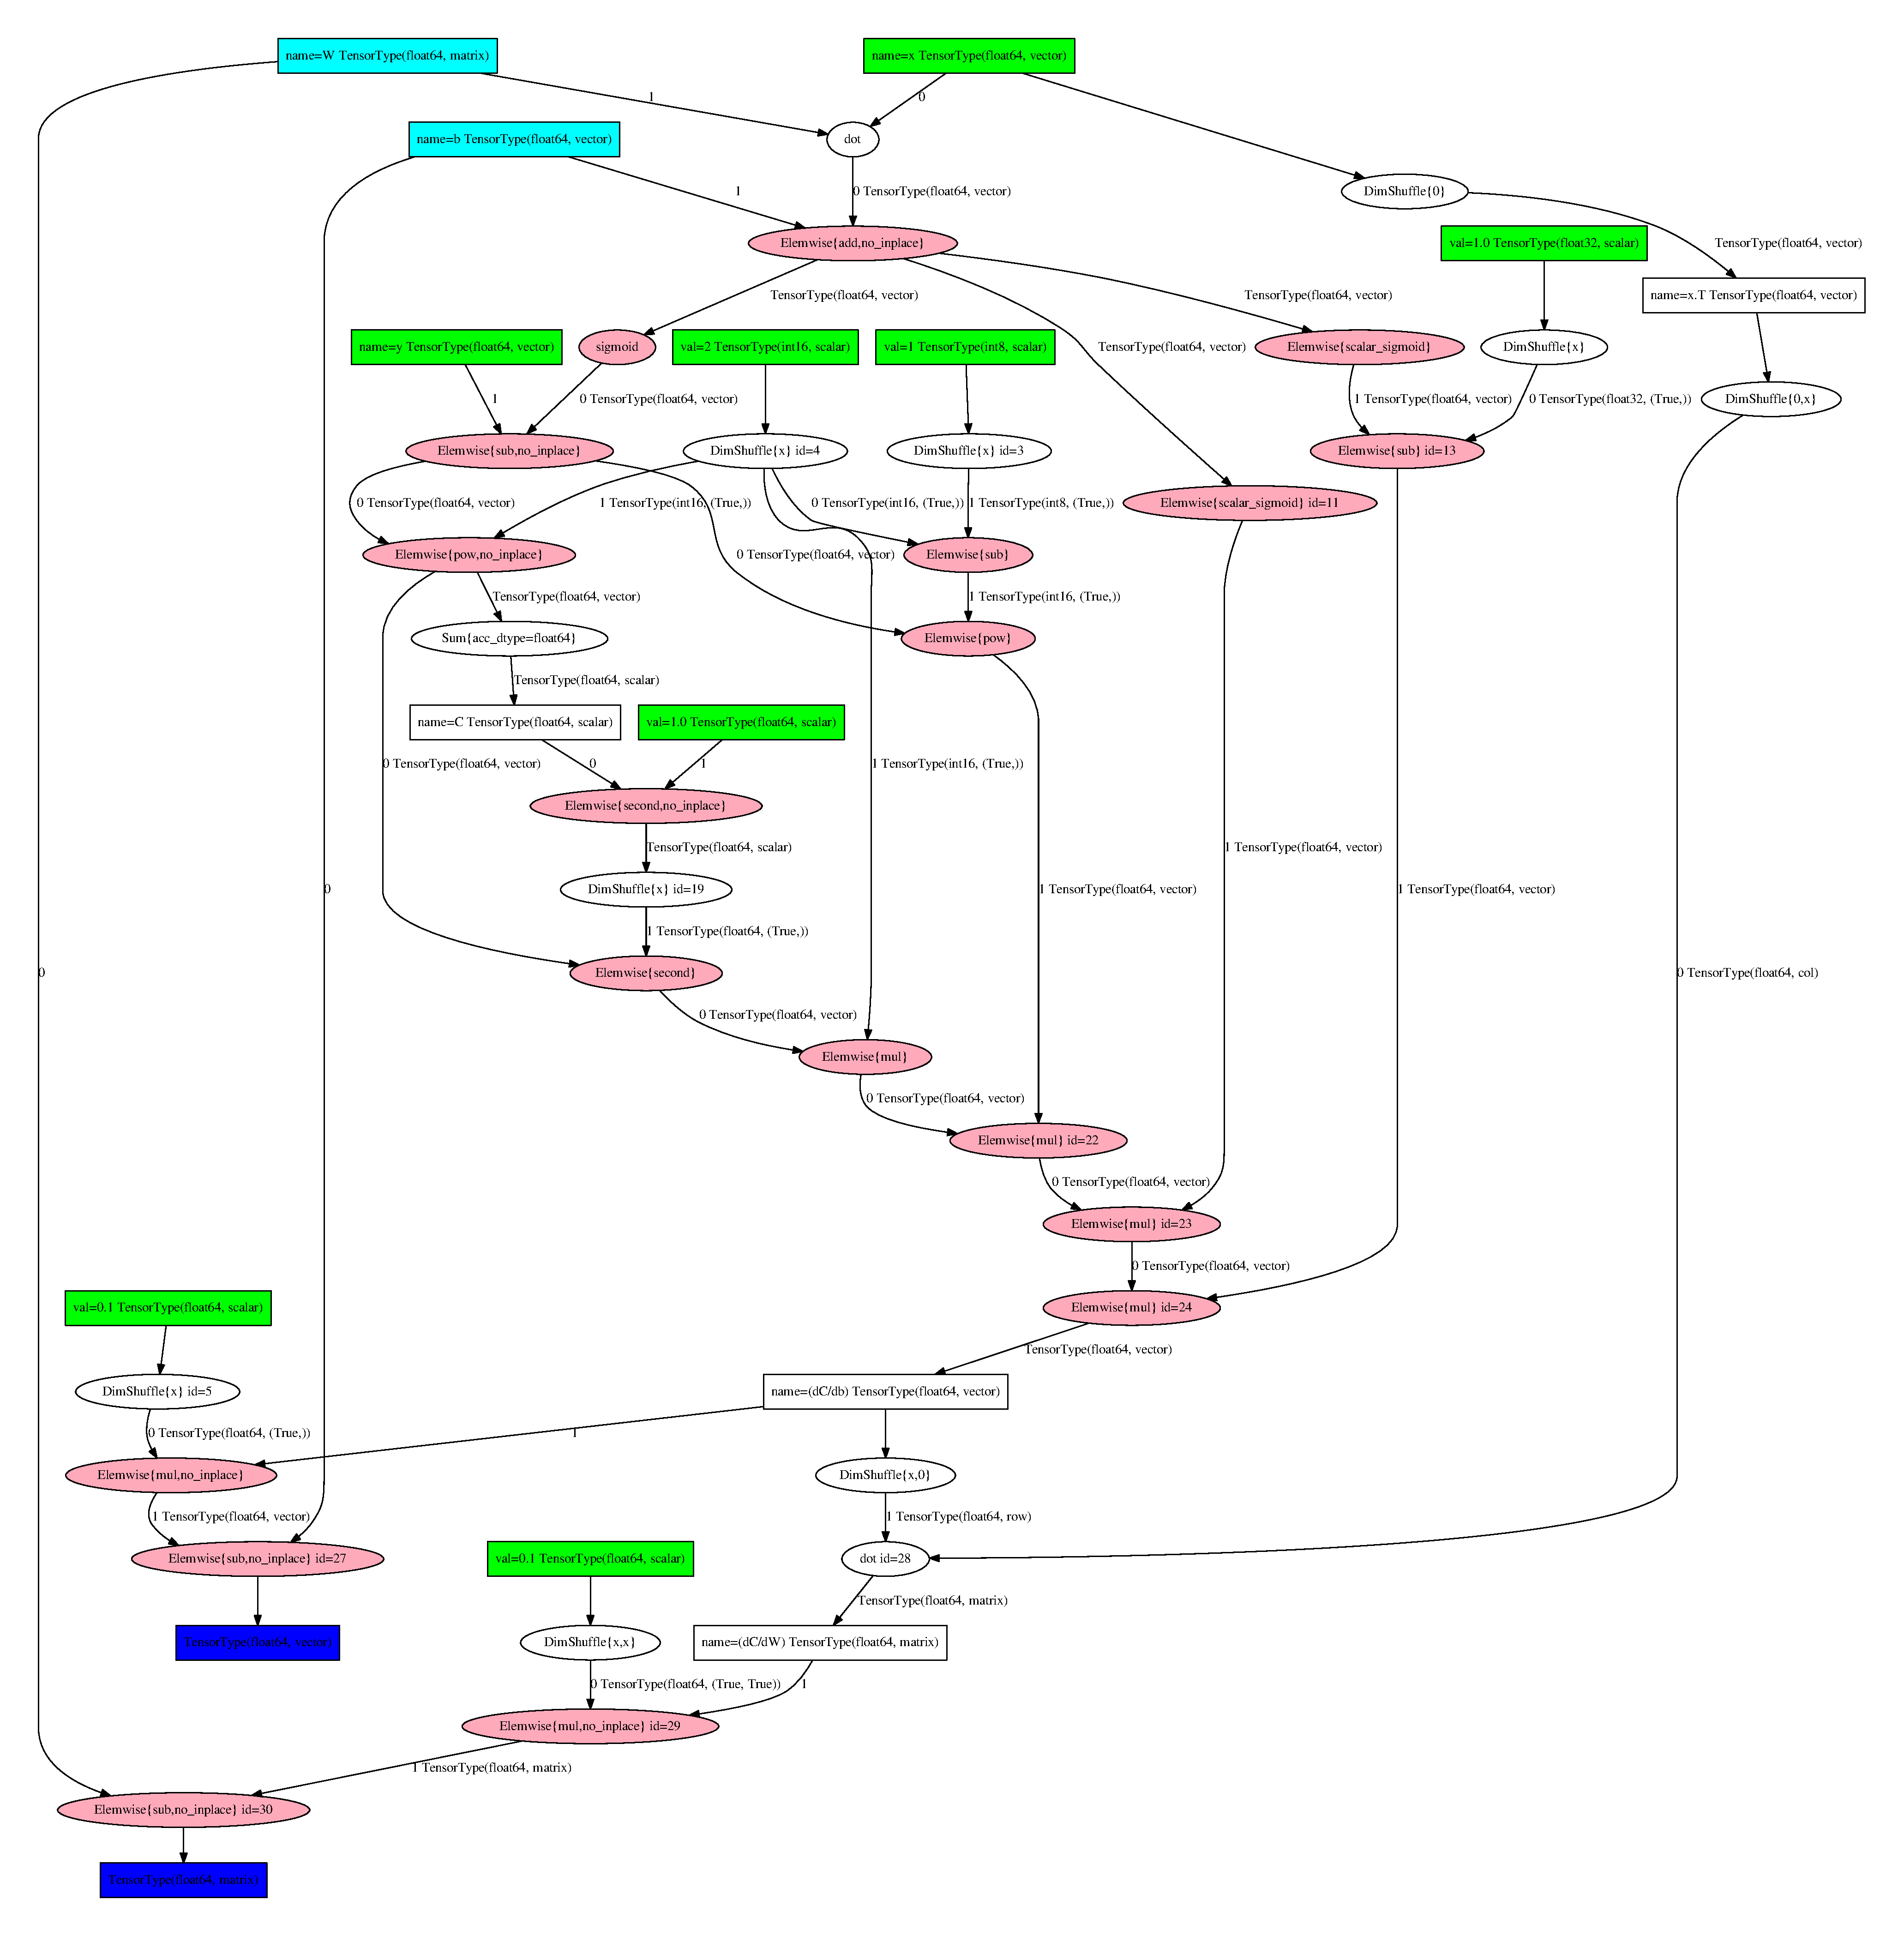
\includegraphics[height=0.9\textheight]{pydotprint_upd.pdf}
\end{frame}


\section{Function compilation}
\begin{frame}
  \tableofcontents[currentsection]
\end{frame}

\subsection{Compiling a Theano function}

\begin{frame}[fragile]{Computing values}
  Build a callable that compute outputs given inputs
  \begin{itemize}
    \item Shared variables are implicit inputs
  \end{itemize}
  \begin{minted}{python}
predict = theano.function([x], out)
x_val = np.random.rand(4)
print(predict(x_val))
# -> array([ 0.9421594 ,  0.73722395,  0.67606977])

monitor = theano.function([x, y], [out, C])
y_val = np.random.uniform(size=3)
print(monitor(x_val, y_val))
# -> [array([ 0.9421594 ,  0.73722395,  0.67606977]),
#     array(0.6137821438190066)]

error = theano.function([out, y], C)
print(error([0.942, 0.737, 0.676], y_val))
# -> array(0.613355628529845)
  \end{minted}
\end{frame}


\begin{frame}[fragile]{Updating shared variables}
  A function can compute new values for shared variables, and perform updates.
  \begin{minted}{python}
train = theano.function([x, y], C,
                        updates=[(W, upd_W),
                                 (b, upd_b)])
print(b.get_value())
# -> [ 1.  1.  1.]
train(x_val, y_val)
print(b.get_value())
# -> [ 0.99639999  0.97684097  0.98318412]
  \end{minted}
  \begin{itemize}
    \item Variables \verb|W| and \verb|b| are {\bf implicit inputs}
    \item Expressions \verb|upd_W| and \verb|upd_b| are {\bf implicit outputs}
    \item All outputs, including the update expressions, are computed {\bf before} the updates are performed
  \end{itemize}
\end{frame}

\subsection{Graph optimizations}

\begin{frame}{Graph optimizations}
  An optimization replaces a part of the graph with different nodes
  \begin{itemize}
    \item The types of the replaced nodes have to match
    \item The values should be equivalent
  \end{itemize}
  Different goals for optimizations:
  \begin{itemize}
    \item Merge equivalent computations
    \item Arithmetic expressions: $x / x$ becomes $1$
    \item Numerical stability: ``$\log (1 + x)$'' becomes ``log1p(x)''
    \item Insert in-place an destructive versions of operations
    \item Use specialized, efficient versions (Elemwise loop fusion, BLAS, cuDNN)
    \item Shape inference
    \item Constant folding
    \item Use of GPU for computations
  \end{itemize}
  \url{http://deeplearning.net/software/theano/optimizations.html}
\end{frame}

\begin{frame}[fragile]{Enabling/disabling optimizations}
  Every time \verb|theano.function| is called, the symbolic relationships between the input and output Theano variables are optimized and compiled. The way this compilation occurs is controlled by the value of the mode parameter.
  \begin{itemize}
    \item \verb|mode='FAST_RUN'|: Apply all optimizations and use C implementations where possible.
    \item \verb|mode='FAST_COMPILE'|: Apply just a few graph optimizations and only use Python implementations. So GPU is disabled.
    \item \verb|mode='DebugMode'|: Verify the correctness of all optimizations, and compare C and Python implementations. This mode can take much longer than the other modes, but can identify several kinds of problems.
    \item \verb|mode='NanGuardMode'|: Same optimization as \verb|FAST_RUN|, but check if a node generate nans.
  \end{itemize}
  
  The default mode is typically \verb|FAST_RUN|, but it can be controlled via the configuration variable \verb|config.mode|, which can be overridden by passing the keyword argument to \verb|theano.function|.

\end{frame}

\subsection{Graph visualization}
\begin{frame}{\texttt{pydotprint(out)}}
    \center
    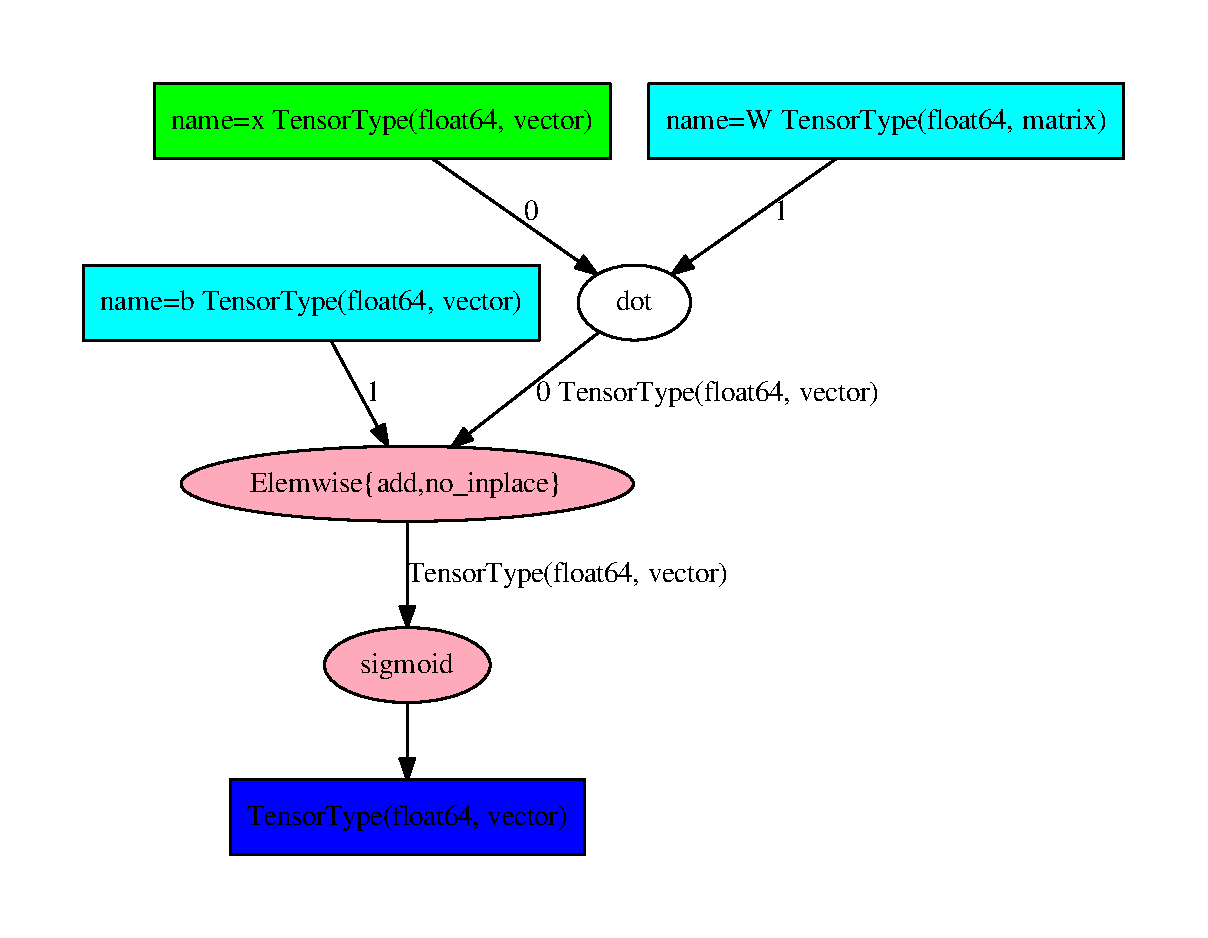
\includegraphics[height=0.9\textheight]{pydotprint_out.pdf}
\end{frame}

\begin{frame}{\texttt{pydotprint(predict)}}
    \center
    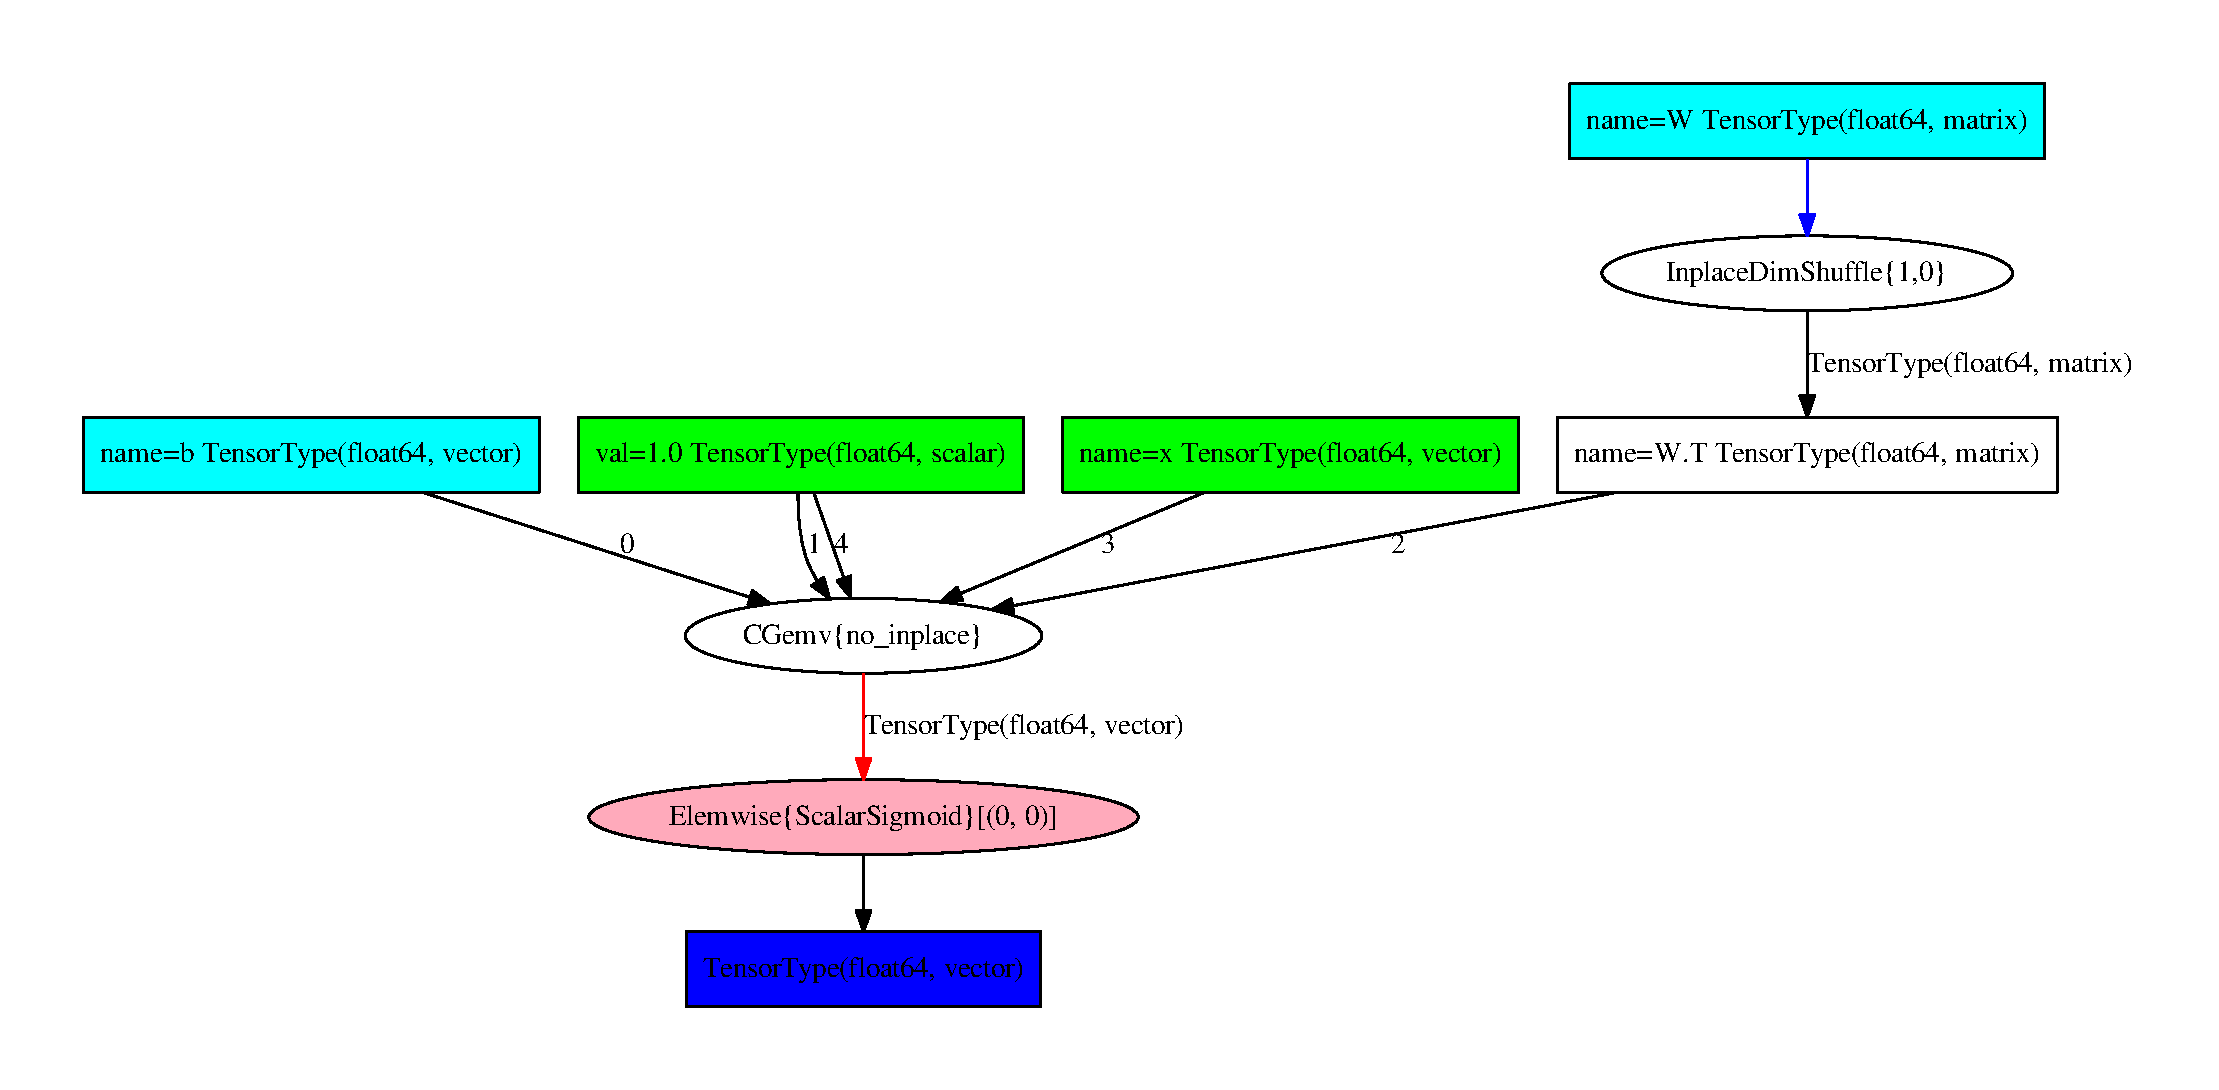
\includegraphics[width=\textwidth]{pydotprint_predict.pdf}
\end{frame}

\begin{frame}{\texttt{pydotprint([upd\_W, upd\_b])}}
    \center
    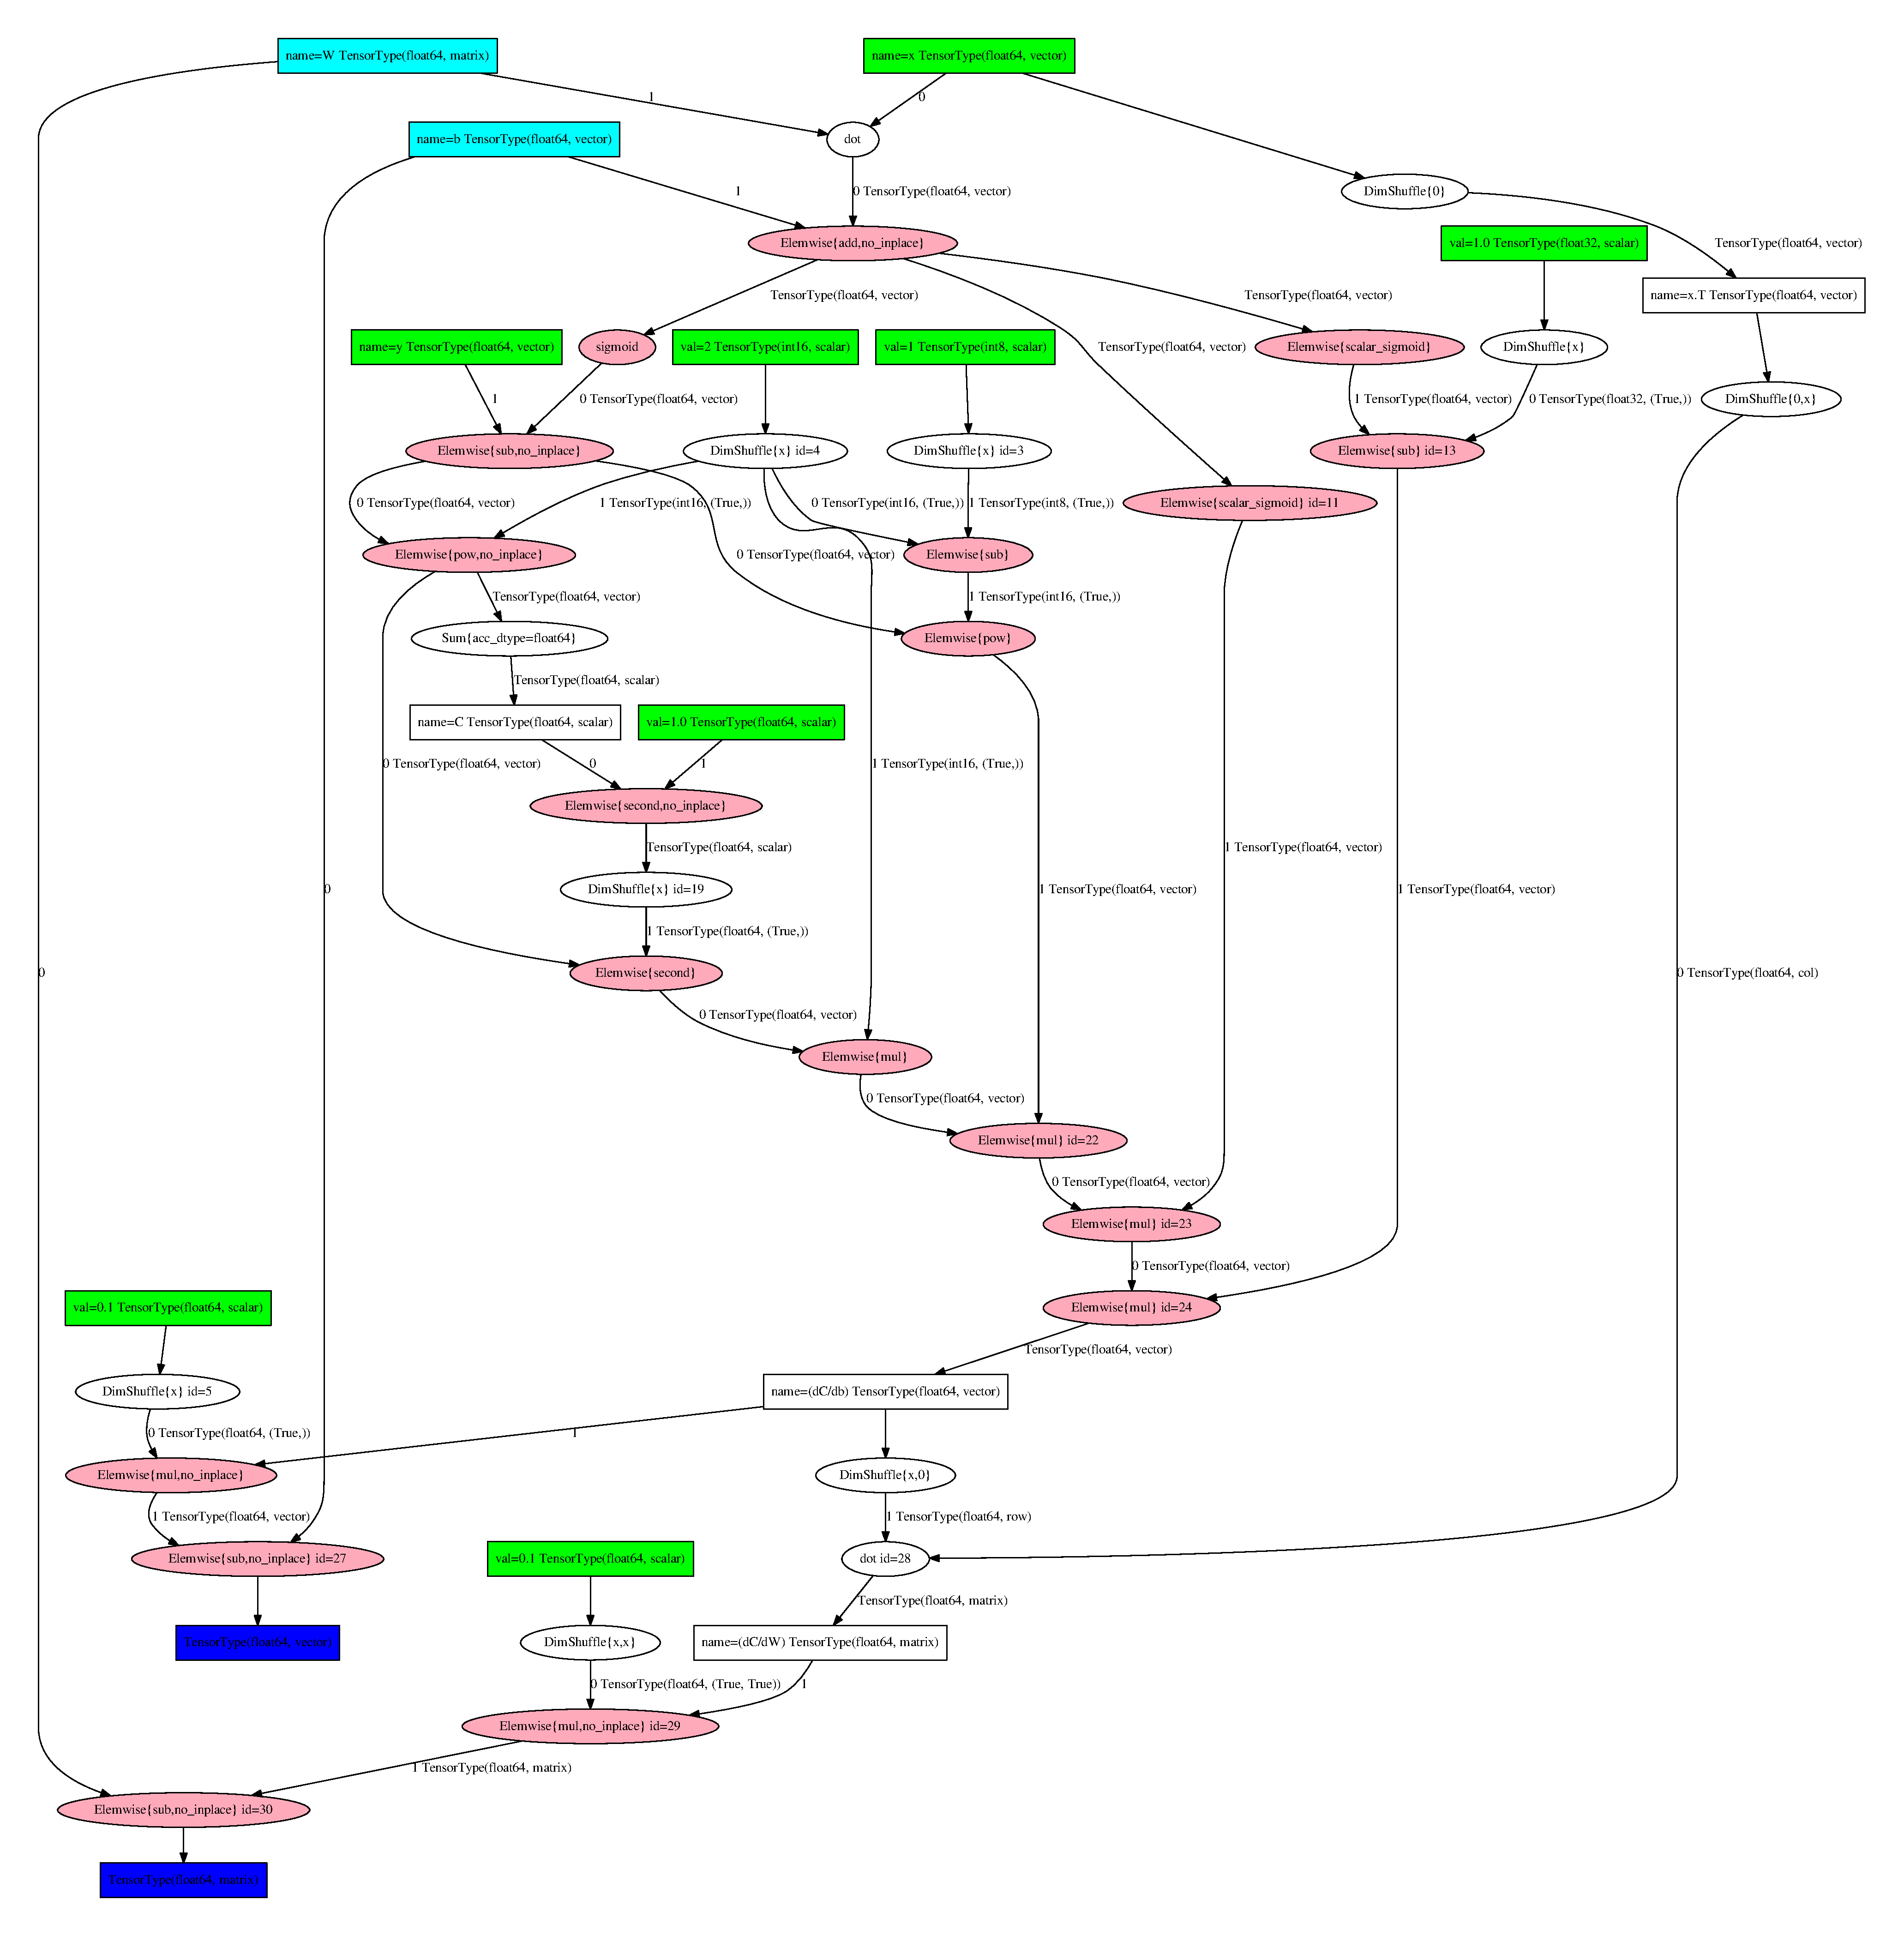
\includegraphics[height=0.9\textheight]{pydotprint_upd.pdf}
\end{frame}

\begin{frame}{\texttt{pydotprint(train)}}
    \center
    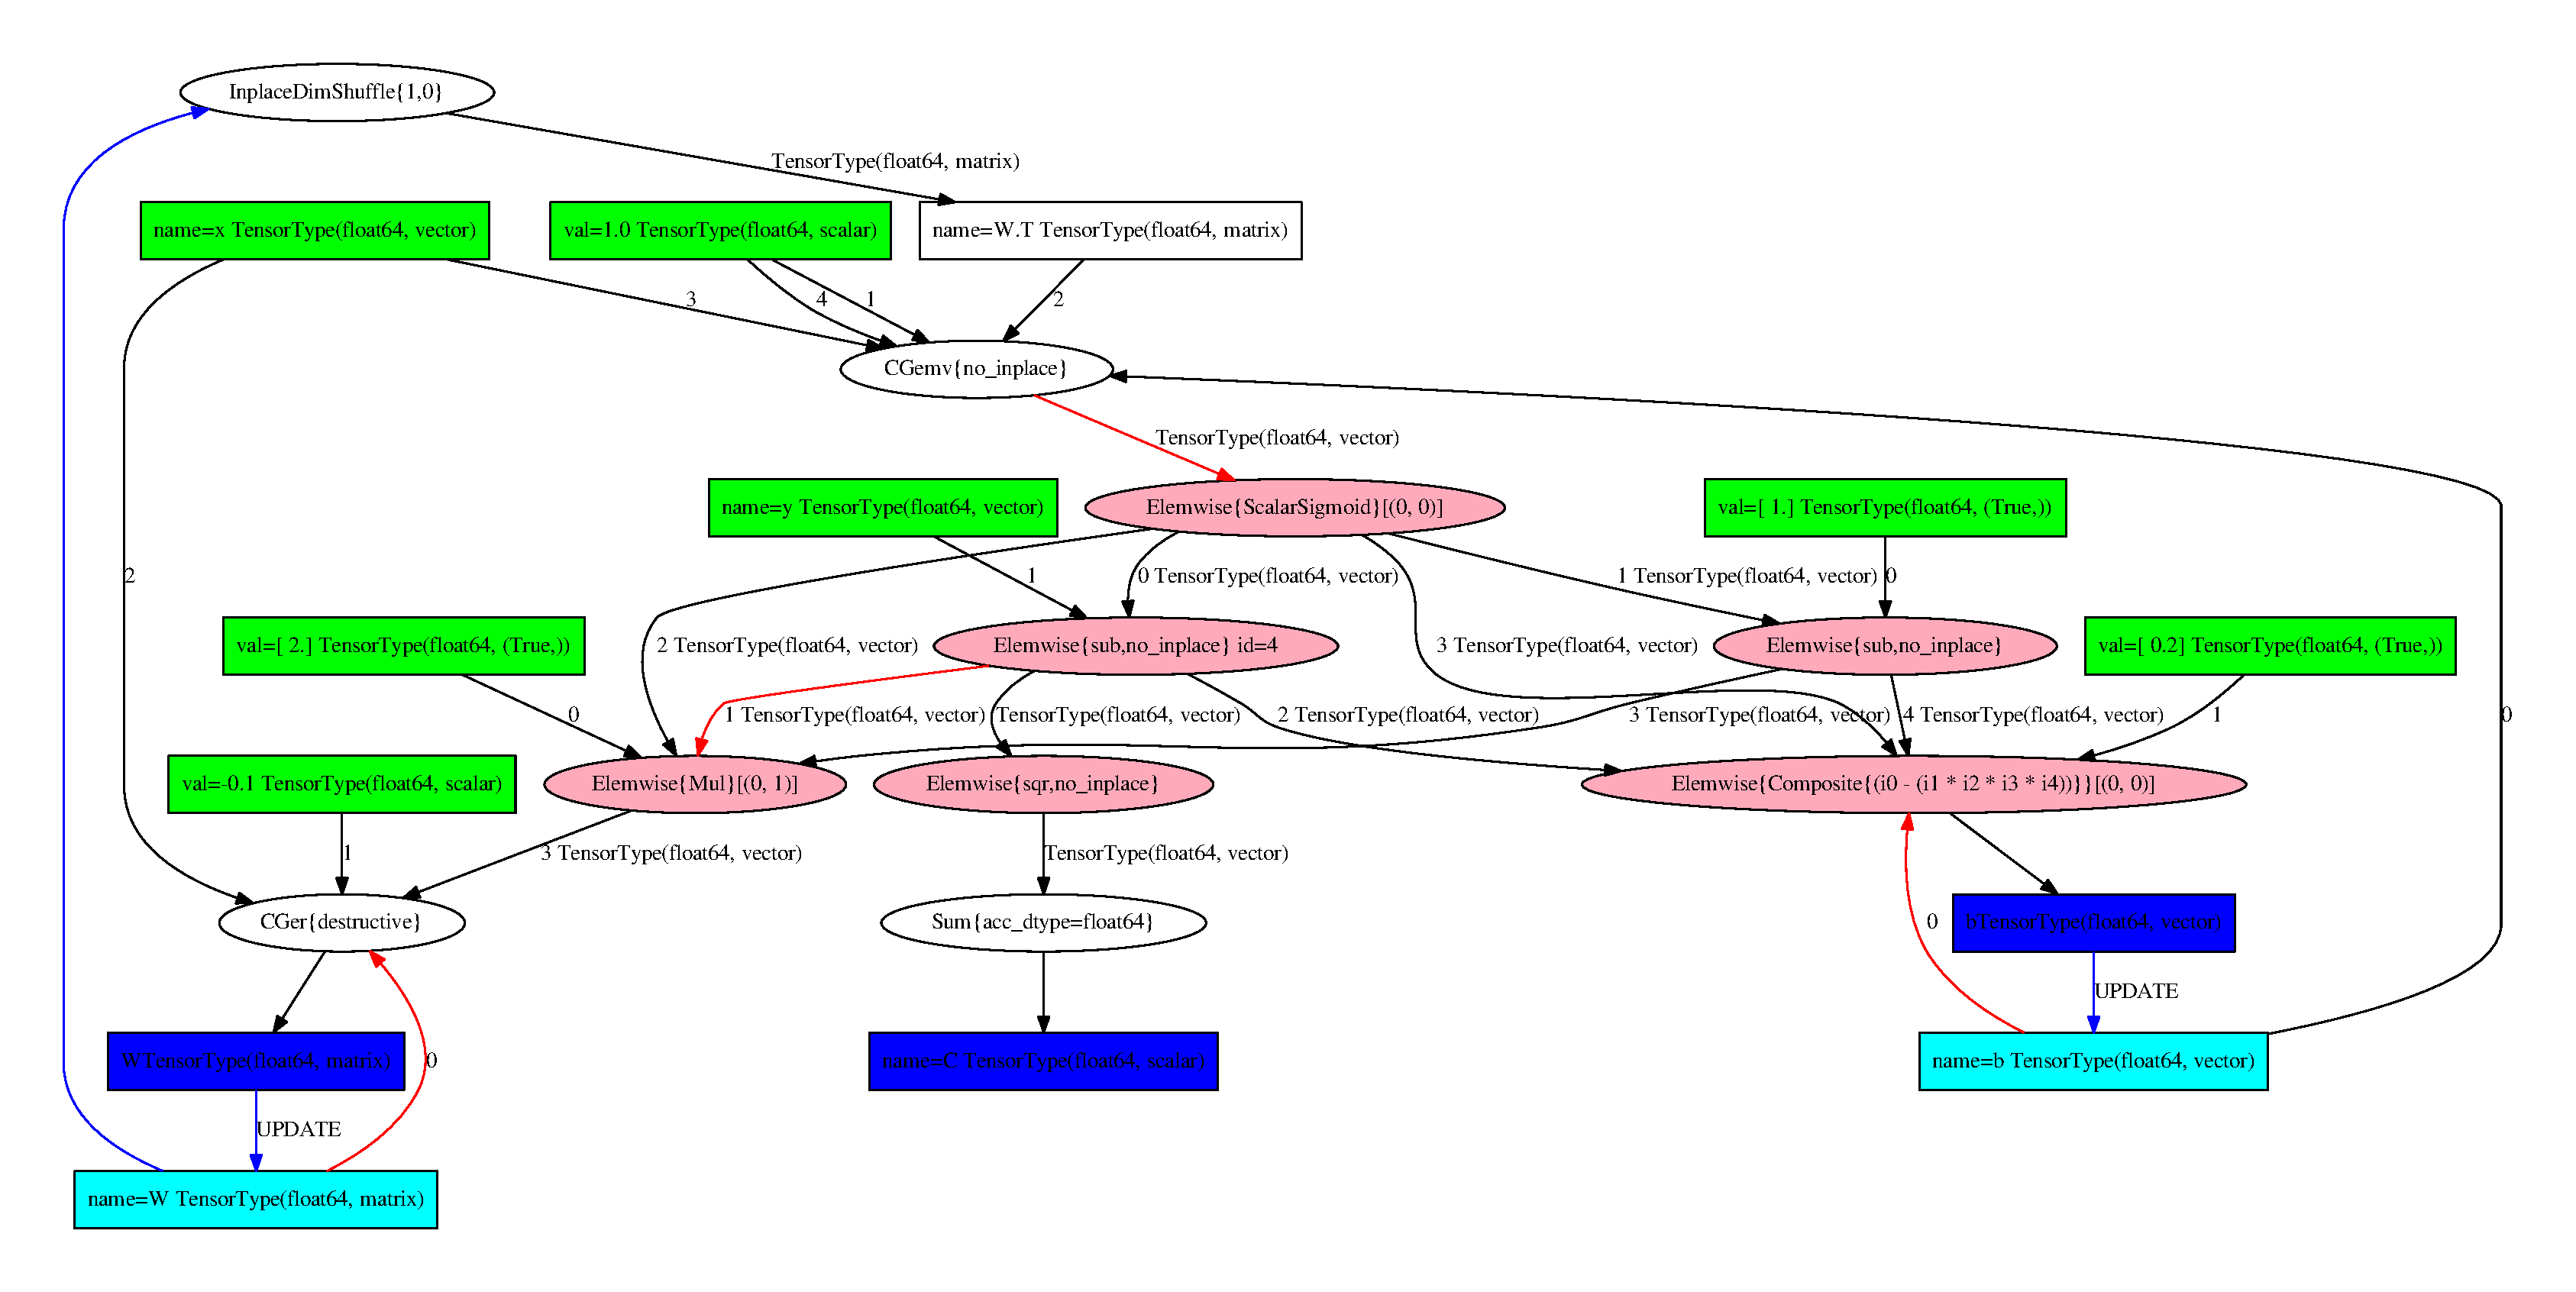
\includegraphics[width=\textwidth]{pydotprint_train.pdf}
\end{frame}


\begin{frame}[fragile]{\texttt{debugprint}}
  \begin{columns}
    \begin{column}{0.45\textwidth}
    \footnotesize
      \begin{verbatim}
debugprint(out)

sigmoid [id A] ''   
 |Elemwise{add,no_inplace} [id B] ''   
   |dot [id C] ''   
   | |x [id D]
   | |W [id E]
   |b [id F]
      \end{verbatim}
    \end{column}

    \begin{column}{0.50\textwidth}
    \footnotesize
      \begin{verbatim}
debugprint(predict)

Elemwise{ScalarSigmoid}[(0, 0)] [id A] ''   2
 |CGemv{no_inplace} [id B] ''   1
   |b [id C]
   |TensorConstant{1.0} [id D]
   |InplaceDimShuffle{1,0} [id E] 'W.T'   0
   | |W [id F]
   |x [id G]
   |TensorConstant{1.0} [id D]
      \end{verbatim}
    \end{column}
  \end{columns}
\end{frame}


\section{Optimized execution}
\begin{frame}
  \tableofcontents[currentsection]
\end{frame}

\subsection{Code generation and execution}
\begin{frame}[fragile]{Code generation and execution}
  Code generation for Ops:
  \begin{itemize}
    \item Ops can define C++/CUDA code computing its output values
    \item Dynamic code generation is possible
      \begin{itemize}
        \item For instance, loop fusion for arbitrary sequence of element-wise operations
      \end{itemize}
    \item Code gets compiled into a Python module, cached, and imported
    \item Otherwise, fall back to a Python implementation
  \end{itemize}

  Code execution through a runtime environment, or VM:
  \begin{itemize}
    \item Calls the functions performing computation for the Ops
    \item Deals with ordering constraints, lazy execution
    \item A C++ implementation (CVM) to avoid context switches
      (in/out of the Python interpreter)
  \end{itemize}
\end{frame}

\subsection{GPU}
\begin{frame}[fragile]{Using the GPU}
  We want to make the use of GPUs as transparent as possible.

  Theano features a new GPU back-end, with
  \begin{itemize}
    \item More dtypes, not only \verb|float32|
    \item Experimental support for \verb|float16| for storage
    \item Easier interaction with GPU arrays from Python
    \item Multiple GPUs and multiple streams
  \end{itemize}

  Select GPU by setting the \verb|device| flag to \verb|'cuda'| or \verb|'cuda{0,1,2,...}'|.
  \begin{itemize}
    \item All {\bf shared} variables will be created in GPU memory by default
    \item Enables optimizations moving supported operations to GPU
    \item Use \verb|float32| for better GPU performance.
  \end{itemize}
\end{frame}

\begin{frame}[fragile]{Configuration flags}
  Configuration flags can be set in a couple of ways:
  \begin{itemize}
    \item In the \verb|.theanorc| configuration file:
      \begin{minted}{text}
[global]
device = cuda0
floatX = float32
      \end{minted}
    \item \verb|THEANO_FLAGS=device=cuda0,floatX=float32| in the shell
    \item In Python:
      \begin{minted}{python}
theano.config.floatX = 'float32'
      \end{minted}
      (\verb|theano.config.device| cannot be set once Theano is imported, but you can call \verb|theano.gpuarray.use('cuda0')|)
  \end{itemize}
\end{frame}


% \section{Advanced Topics}
% \begin{frame}
%   \tableofcontents[currentsection]
% \end{frame}

% \subsection{Looping: the \texttt{scan} operation}
% \begin{frame}[fragile]{Overview of \texttt{scan}}
%   Symbolic looping
%   \begin{itemize}
%     \item Can perform map, reduce, reduce and accumulate, \ldots
%     \item Can access outputs at previous time-step, or further back
%     \item Symbolic number of steps
%     \item Symbolic stopping condition (behaves as \verb|do ... while|)
%     \item Actually embeds a small Theano function
%     \item Gradient through \verb|scan| implements backprop through time
%     \item Can be transfered to GPU
%   \end{itemize}
% \end{frame}

% \begin{frame}[fragile]{Example: Loop with accumulation}
%   \footnotesize
%     \begin{minted}{python}
% k = T.iscalar("k")
% A = T.vector("A")

% # Symbolic description of the result
% result, updates = theano.scan(fn=lambda prior_result, A: prior_result * A,
%                               outputs_info=T.ones_like(A),
%                               non_sequences=A,
%                               n_steps=k)

% # We only care about A**k, but scan has provided us with A**1 through A**k.
% # Discard the values that we don't care about. Scan is smart enough to
% # notice this and not waste memory saving them.
% final_result = result[-1]

% # compiled function that returns A**k
% power = theano.function(inputs=[A, k], outputs=final_result, updates=updates)

% print(power(range(10), 2))
% # [  0.   1.   4.   9.  16.  25.  36.  49.  64.  81.]
% print(power(range(10), 4))
% # [  0.00000000e+00   1.00000000e+00   1.60000000e+01   8.10000000e+01
% #    2.56000000e+02   6.25000000e+02   1.29600000e+03   2.40100000e+03
% #    4.09600000e+03   6.56100000e+03]
%   \end{minted}
% \end{frame}

% \subsection{Debugging}
% \begin{frame}[fragile]{Visualization, debugging, and diagnostic tools}
%   The \emph{definition} of a Theano function is separate from its \emph{execution}.
%   To help with this, we provide:
%   \begin{itemize}
%     \item Information in error messages
%     \item Get information at runtime
%     \item Monitor NaN or large value
%     \item Test values when building the graph
%     \item Detect common sources of slowness
%     \item Self-diagnostic tools
%   \end{itemize}
% \end{frame}

% \subsection{Extending Theano}

% \begin{frame}{Extending Theano}
% Theano can be extended in a few different ways
%   \begin{itemize}
%     \item Creating an Op with Python code
%       \begin{itemize}
%         \item Easy, using Python bindings for specialized libraries (PyCUDA, \ldots)
%         \item Some runtime overhead is possible
%         \item Example: 3D convolution using FFT on GPU
%       \end{itemize}
%     \item Creating an Op with C or CUDA code
%       \begin{itemize}
%         \item Use the C-API of Python / NumPy / GpuArray, manage refcounts
%         \item No overhead of Python function calls, or from the interpreter
%         \item C++ code inline or in a separate file
%         \item Example: Caffe-style convolutions, using GEMM, on CPU and GPU
%       \end{itemize}
%     \item Adding an optimization
%       \begin{itemize}
%         \item Perform additional graph simplifications
%         \item Replace part of the graph by a new optimized Op
%       \end{itemize}
%   \end{itemize}
% \end{frame}


% \subsection{Development}

% \begin{frame}[fragile]{New features}
%   \begin{itemize}
%     \item New GPU back-end, based on \verb|libgpuarray|, with:
%       \begin{itemize}
%         \item Arrays of all dtypes, half-precision float (\verb|float16|) for storage
%         \item Better scheduling
%         \item Much simpler installation on Windows (conda package)
%       \end{itemize}
%     \item Performance improvements
%       \begin{itemize}
%         \item Integration of CuDNN (now v6) for 2D/3D convolutions and pooling, RNNs, batch normalization
%         \item Fast memory allocator on GPU
%         \item For memory: checkpointing in scan, gradients of long sequences
%         \item Data parallelism with Platoon (\url{github.com/mila-udem/platoon/})
%       \end{itemize}
%     \item Faster graph optimization phase
%       \begin{itemize}
%         \item More optimization / compile time trade-offs (\verb|optimizer={o0,o1,...,o4}|)
%         \item Various ways to avoid recompilation
%       \end{itemize}
%     \item Diagnostic tools
%       \begin{itemize}
%         \item Interactive visualization (d3viz)
%         \item \verb|PdbBreakPoint|
%       \end{itemize}
%   \end{itemize}
% \end{frame}

% \begin{frame}[fragile]{Current development}
%   \begin{itemize}
%     \item Better support for int operations on GPU (indexing, argmax)
%     \item Faster reductions on GPU
%     \item Simpler, faster optimization mode
%     \item Faster generation and loading of C++ / CUDA code
%     \item More convolution variants: grouped, dilated, \ldots (GSoC)
%     \item More linear algebra operations on GPU (GSoC)
%     \item Data parallelism across nodes in Platoon
%     \item \verb|OpFromGraph| for re-defining gradients
%   \end{itemize}
% \end{frame}

% \begin{frame}[fragile]{Projects in our road map}
%   \begin{itemize}
%     \item Constant shape inference when building the graph
%     \item Better compilation cache for generated C++ code
%     \item Continue refactoring graph optimization (for optimization speed)
%     \item Optimize and re-use sub-graphs (like subroutines)
%       \begin{itemize}
%         \item Improving \verb|OpFromGraph|
%         \item Maybe cache them
%       \end{itemize}
%     \item Deterministic mode
%     \item Use CPU memory to offload intermediate results from GPU (maybe limited to Pascal GPUs)
%   \end{itemize}
% \end{frame}

% \subsection{Lasagne}

% \begin{frame}{What is Lasagne?}
%   Lasagne is a thin framework/library on top of Theano.
%   \url{lasagne.readthedocs.org}
%   \begin{itemize}
%     \item Does not hide Theano
%     \item Builds Theano graphs easily by using layers
%     \item Contains many preimplemented losses and optimizers
%     \item Does not include a training loop
%   \end{itemize}
% \end{frame}


% \section{}

% \begin{frame}{Acknowledgements}
%   \begin{itemize}
%     \item All people working or having worked at the MILA (previously LISA), especially Theano contributors
%       \begin{itemize}
%         \item
%           Reyhane Askari Hemmat,
%           Frédéric Bastien,
%           Yoshua Bengio,
%           James Bergstra,
%           Arnaud Bergeron,
%           Steven Bocco,
%           Philemon Brakel,
%           Olivier Breuleux,
%           Pierre Luc Carrier,
%           Mathieu Germain,
%           Ian Goodfellow,
%           Simon Lefrançois,
%           Razvan Pascanu,
%           Joseph Turian,
%           David Warde-Farley,
%           and many more
%       \end{itemize}
%     \item Compute Canada, Calcul Québec, NSERC, the Canada Research Chairs, CIFAR, and the CFI for providing funding or access to compute resources
%     \item CIFAR and CRM for organizing the Deep learning summer school
%   \end{itemize}
% \end{frame}

\section{Case Study}
\subsection{Logistic Regression}
\begin{frame}[fragile]{Logistic Regression-I}


\begin{minted}{python}
import numpy
import theano
import theano.tensor as T
rng = numpy.random

N = 400         # training sample size
feats = 784     # number of input variables

# generate a dataset: D = (input_values, target_class)
D = (rng.randn(N, feats), rng.randint(size=N, low=0, high=2))
training_steps = 10000

# Declare Theano symbolic variables
x = T.dmatrix("x")
y = T.dvector("y")

\end{minted}
\end{frame}

\begin{frame}[fragile]{Logistic Regression-II}
\begin{minted}{python}
# initialize the weight vector w randomly
# weight w and bias variable b are shared 
# so they keep their values between 
# training iterations (updates)
w = theano.shared(rng.randn(feats), name="w")

# initialize the bias term
b = theano.shared(0., name="b")

print("Initial model:")
print(w.get_value())
print(b.get_value())

\end{minted}
\end{frame}


\begin{frame}[fragile]{Logistic Regression-III}
\begin{minted}{python}
# Construct Theano expression graph

# Probability that target = 1
p_1 = 1 / (1 + T.exp(-T.dot(x, w) - b))

# The prediction thresholded
prediction = p_1 > 0.5

# Cross-entropy loss function
xent = -y * T.log(p_1) - (1-y) * T.log(1-p_1)

# The cost to minimize
cost = xent.mean() + 0.01 * (w ** 2).sum()

# Compute the gradient of the cost w.r.t weight vector w and bias term b
gw, gb = T.grad(cost, [w, b])             
\end{minted}
\end{frame}


\begin{frame}[fragile]{Logistic Regression-IV}
\begin{minted}{python}
# Compile
train = theano.function(
          inputs=[x,y],
          outputs=[prediction, xent],
          updates=((w, w - 0.1 * gw), (b, b - 0.1 * gb)))
predict = theano.function(inputs=[x], outputs=prediction)

# Train
for i in range(training_steps):
    pred, err = train(D[0], D[1])

print("Final model:")
print(w.get_value())
print(b.get_value())
print("target values for D:")
print(D[1])
print("prediction on D:")
print(predict(D[0]))
\end{minted}
\end{frame}


\section{}
\subsection{}
\begin{frame}[fragile]{Thanks for your attention}

The End!!!
%   \uncover<1->{%
%     Questions, comments, requests?
%   }
%   \vspace{.5cm}

%   \uncover<2->{%
%     \url{github.com/mila-udem/summerschool2017}
%     \begin{itemize}
%       \item Slides: {\tt theano.pdf}
%       \item Companion notebook: {\tt notebooks/intro\_theano.ipynb}
%     \end{itemize}
%   }

%   \vspace{.5cm}
%   \uncover<3->{%
%     More resources
%     \begin{itemize}
%       \item Documentation: \url{deeplearning.net/software/theano/}
%       \item Code: \url{github.com/Theano/Theano/}
%       \item Article: The Theano Development Team, ``Theano: A Python framework for fast computation of mathematical expressions'', \url{arxiv.org/abs/1605.02688}
%       \item Deep Learning Tutorials: \url{deeplearning.net/tutorial/}
%     \end{itemize}
%   }
\end{frame}

% \begin{frame}[fragile]{Examples}

%   Go to \url{http://mila.umontreal.ca/vmip}

% \end{frame}


\end{document}
